The results chapter is split into three parts to match the sections of the post-test questionnaire: VR sickness (see question 2 in Appendix B), presence (see questions 3-8 in Appendix B), and usability (see question 9 in Appendix B). This study employed a repeated measures design, where each of 20 participants tested in succession all four solutions to the problem of VR head collisions. For each solution, 20 results were gathered from the questionnaires. If the assumptions of normality and sphericity were not violated, the difference between means were analyzed at 0.05 level of significance using a repeated measures ANOVA; otherwise, a Friedman test was used. The distribution of the data was checked for normality using a Shapiro-Wilk test, and a Mauchly's test was used to assess sphericity. If the results indicated statistical significance, additional post-hoc tests with Bonferroni correction were used to determine which means differed from each other. All tests were performed in MATLAB (version R2015a) \cite{MATLAB}.

\section{VR Sickness}

\subsection{Nausea, Oculomotor, and Disorientation}

The SSQ nausea, oculomotor, and disorientation scores were calculated and were analyzed using Friedman tests due to non-normality. The method of handling collisions did not significantly influence the SSQ nausea scores (\textit{$\chi\textsuperscript{2}$}(3) = 4.536, \textit{p} = 0.209) and the SSQ oculomotor scores (\textit{$\chi\textsuperscript{2}$}(3) = 7.173, \textit{p} = 0.067). The test revealed that the SSQ disorientation scores were significantly influenced by the method (\textit{$\chi\textsuperscript{2}$}(3) = 8.713, \textit{p} = 0.033). Post-hoc Wilcoxon signed-rank tests revealed that the screen fade method led to significantly lower scores than the delayed push-back method (\textit{p} = 0.017). See Figure \ref{fig:ssq_secondary} for an overview of the SSQ nausea, oculomotor, and disorientation scores.

\begin{figure}[ph]
\centering
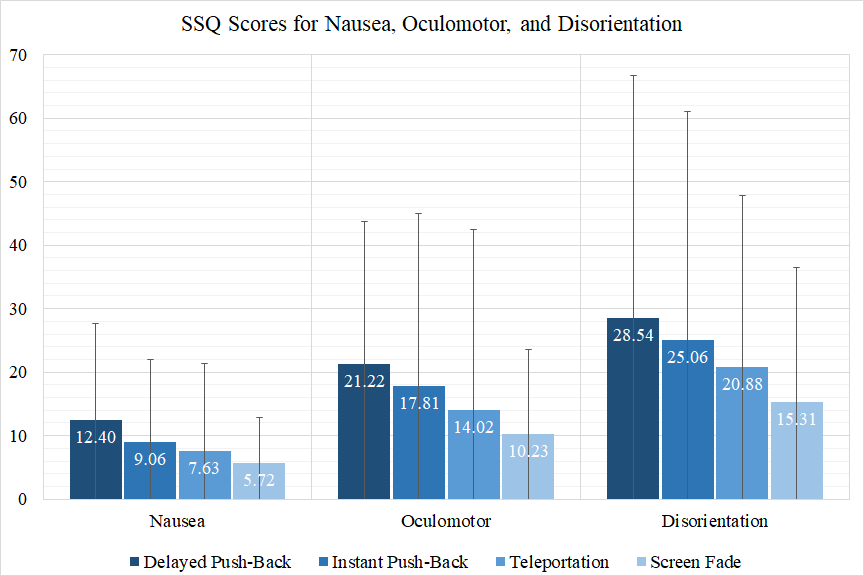
\includegraphics[width=1\textwidth]{img/ssq_secondary.png}
\caption{The SSQ scores for nausea, oculomotor, and disorientation.}
\label{fig:ssq_secondary}
\end{figure}

\subsection{Total SSQ Scores}

The total SSQ scores were calculated and were analyzed using a Friedman test due to non-normality. The test revealed that the total SSQ scores were significantly influenced by the method of handling collisions (\textit{$\chi\textsuperscript{2}$}(3) = 9.881, \textit{p} = 0.02). Post-hoc Wilcoxon signed-rank tests revealed that the screen fade method led to significantly lower scores than the delayed push-back method (\textit{p} < 0.001). See Figure \ref{fig:ssq_total} for an overview of the total SSQ scores.

\begin{figure}[ph]
\centering
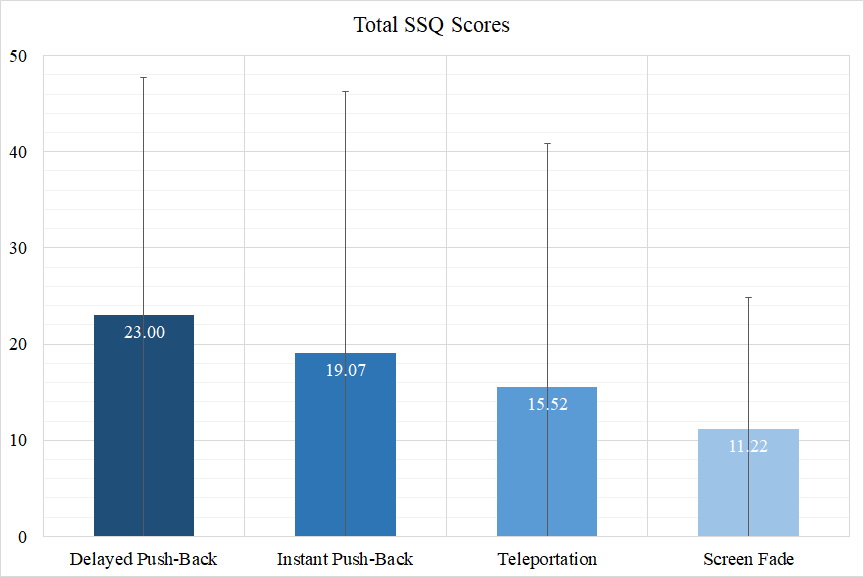
\includegraphics[width=1\textwidth]{img/ssq_total.png}
\caption{The total SSQ scores.}
\label{fig:ssq_total}
\end{figure}

\section{Sense of Presence}

The SUS presence scores were calculated by counting a number of answers to questions 3-8 that have a score of 6 or 7. Shapiro-Wilk tests
indicated that the assumption of normality was not violated; and Mauchly's test indicated that the assumption of sphericity was met (\textit{$\chi\textsuperscript{2}$}(3) = 9.758, \textit{p} = 0.082). A repeated measures ANOVA revealed that the presence scores were significantly influenced by the method of handling collisions (\textit{F}(3, 76) = 11, \textit{p} < 0.00001). Post-hoc pairwise comparisons revealed higher presence scores for the screen fade method compared to the delayed push-back (\textit{p} < 0.001) and teleportation (\textit{p} = 0.002). The comparisons also revealed higher presence scores for the instant push-back method compared to the delayed push-back method (\textit{p} = 0.01). See Figure \ref{fig:presence_scores} for an overview of the SUS presence scores.

\begin{figure}[th]
\centering
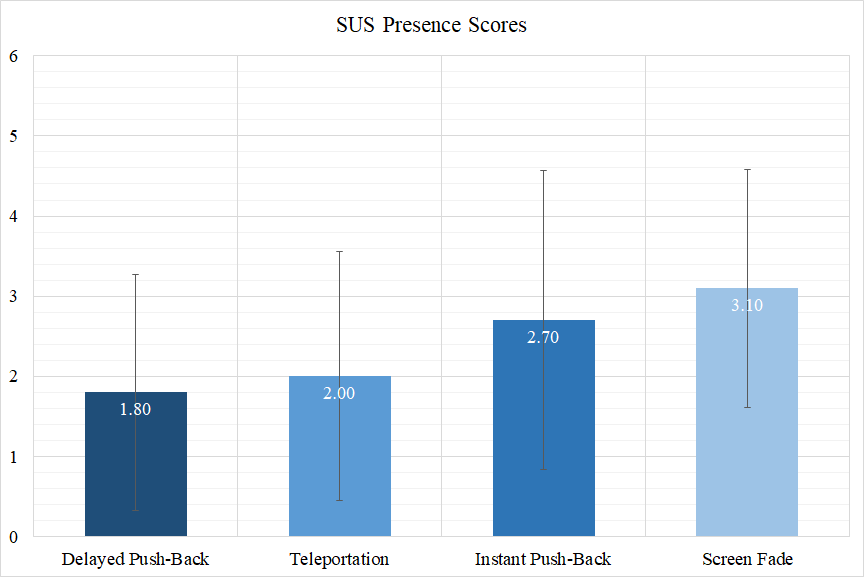
\includegraphics[width=1\textwidth]{img/presence_scores.png}
\caption{The SUS presence scores.}
\label{fig:presence_scores}
\end{figure}

\section{Usability}

\subsection{Difficulty in Understanding and Operating}

The usability scores for difficulty in understanding and operating the method were analyzed using Friedman tests due to non-normality. The method of handling collisions did not significantly influence the scores for difficulty in understanding (\textit{$\chi\textsuperscript{2}$}(3) = 7.359, \textit{p} = 0.061) and the scores for difficulty in operating (\textit{$\chi\textsuperscript{2}$}(3) = 6.788, \textit{p} = 0.079). See Figure \ref{fig:difficulty_scores} for an overview of the usability scores for difficulty in understanding and operating the method.

\begin{figure}[th]
\centering
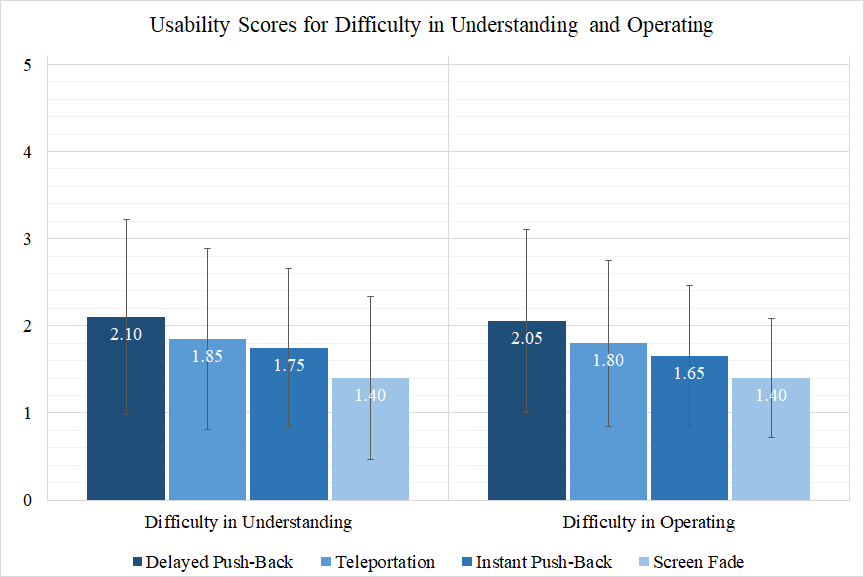
\includegraphics[width=1\textwidth]{img/difficulty_scores.png}
\caption{The usability scores for difficulty in understanding and operating the method.}
\label{fig:difficulty_scores}
\end{figure}

\subsection{Required Effort and Tiredness}

The usability scores for required effort and tiredness while using the method were analyzed using Friedman tests due to non-normality. The method of handling collisions did not significantly influence the scores for required effort (\textit{$\chi\textsuperscript{2}$}(3) = 5.057, \textit{p} = 0.168). However, the tests revealed that the scores for tiredness were significantly influenced by the method (\textit{$\chi\textsuperscript{2}$}(3) = 11.231, \textit{p} = 0.011). Post-hoc Wilcoxon signed-rank tests revealed that the screen fade method led to significantly lower scores for tiredness than the delayed push-back method (\textit{p} = 0.007). See Figure \ref{fig:effort_tiredness_scores} for an overview of the usability scores for required effort and tiredness while using the method.

\begin{figure}[ph]
\centering
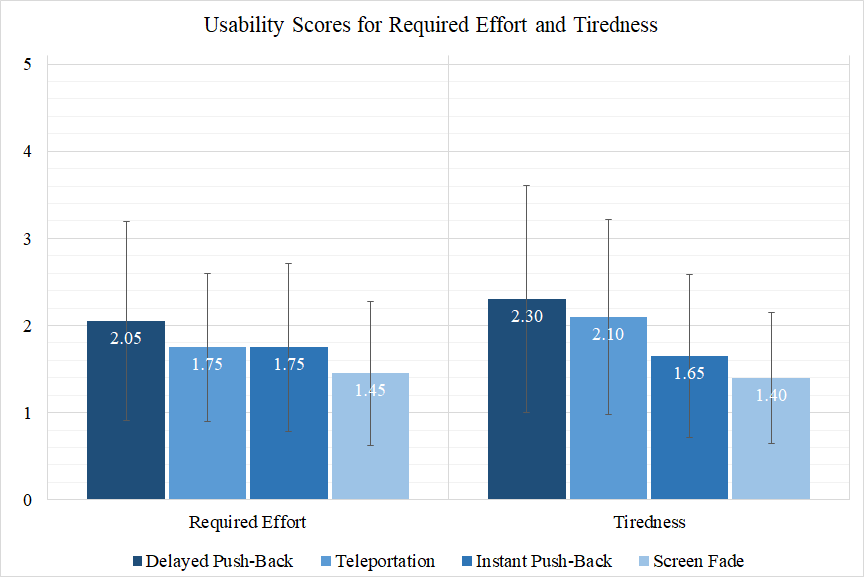
\includegraphics[width=1\textwidth]{img/effort_tiredness_scores.png}
\caption{The usability scores for required effort and tiredness while using the method.}
\label{fig:effort_tiredness_scores}
\end{figure}

\subsection{Feeling of Being in Control and Enjoyment}

The usability scores for the feeling of being in control and enjoyment while using the method were analyzed using Friedman tests due to non-normality. The method of handling collisions significantly influenced the scores for the feeling of being in control (\textit{$\chi\textsuperscript{2}$}(3) = 5.057. Post-hoc Wilcoxon Signed Rank tests revealed that the instant push-back method led to significantly higher scores for the feeling of being in control than the delayed push-back method (\textit{p} = 0.002). The Friedman tests also revealed that the scores for enjoyment were significantly influenced by the method (\textit{$\chi\textsuperscript{2}$}(3) = 16.297, \textit{p} < 0.001). Post-hoc Wilcoxon signed-rank tests revealed that the screen fade method led to significantly higher scores for enjoyment than the delayed push-back (\textit{p} = 0.003) and teleportation (\textit{p} = 0.004). See Figure \ref{fig:incontrol_enjoyment_scores} for an overview of the usability scores for the feeling of being in control and enjoyment while using the method.

\begin{figure}[ph]
\centering
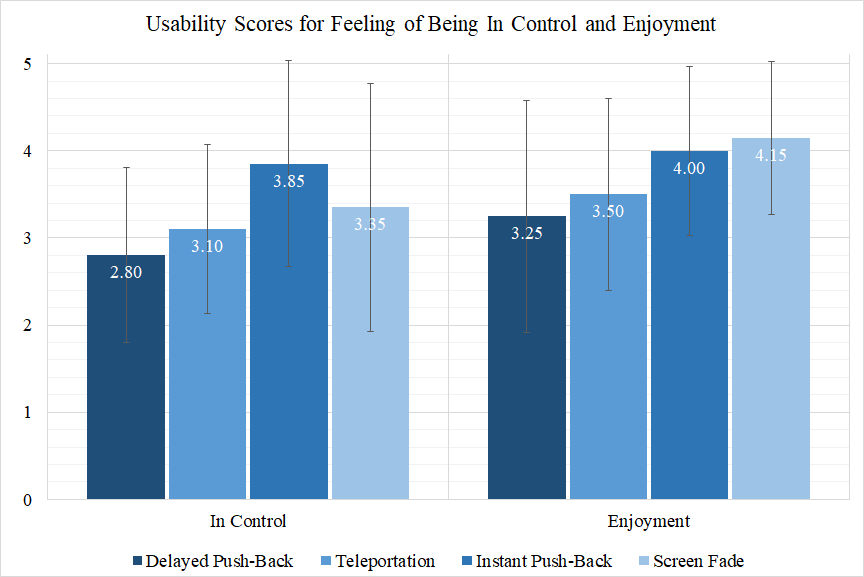
\includegraphics[width=1\textwidth]{img/incontrol_enjoyment_scores.png}
\caption{The usability scores for the feeling of being in control and enjoyment while using the method.}
\label{fig:incontrol_enjoyment_scores}
\end{figure}

\subsection{Feeling of Being Overwhelmed and Frustration}

The usability scores for the feeling of being overwhelmed and frustration while using the method were analyzed using Friedman tests due to non-normality. The method of handling collisions did not significantly influence the scores for the feeling of being overwhelmed (\textit{$\chi\textsuperscript{2}$}(3) = 3.675, \textit{p} = 0.299). However, the tests revealed that the scores for frustration were significantly influenced by the method (\textit{$\chi\textsuperscript{2}$}(3) = 13.227, \textit{p} = 0.004). Post-hoc Wilcoxon signed-rank tests revealed that the screen fade method led to significantly lower scores for frustration than the delayed push-back method (\textit{p} = 0.004). See Figure \ref{fig:overwhelm_frustration_scores} for an overview of the usability scores for the feeling of being overwhelmed and frustration while using the method.

\begin{figure}[th]
\centering
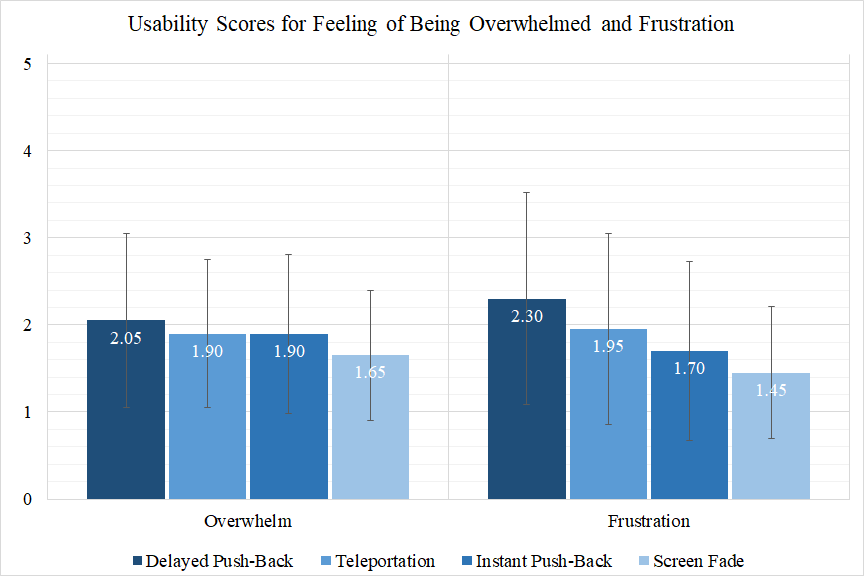
\includegraphics[width=1\textwidth]{img/overwhelm_frustration_scores.png}
\caption{The usability scores for the feeling of being overwhelmed and frustration while using the method.}
\label{fig:overwhelm_frustration_scores}
\end{figure}

\subsection{Total Usability Scores}

The total usability scores were calculated and were analyzed using a repeated measures ANOVA. Shapiro-Wilk tests indicated that the assumption of normality was not violated; and Mauchly's test indicated that the assumption of sphericity was met (\textit{$\chi\textsuperscript{2}$}(3) = 8.08, \textit{p} = 0.152). The repeated measures ANOVA revealed that the total usability scores were significantly influenced by the method of handling collisions (\textit{F}(3, 76) = 8.887, \textit{p} < 0.0001). Post-hoc pairwise comparisons revealed higher usability scores for the screen fade method compared to the delayed push-back (\textit{p} = 0.005) and teleportation (\textit{p} = 0.021). The comparisons also revealed higher usability scores for the instant push-back method compared to the delayed push-back method (\textit{p} = 0.03). See Figure \ref{fig:total_usability_scores} for an overview of the total usability scores.

\begin{figure}[th]
\centering
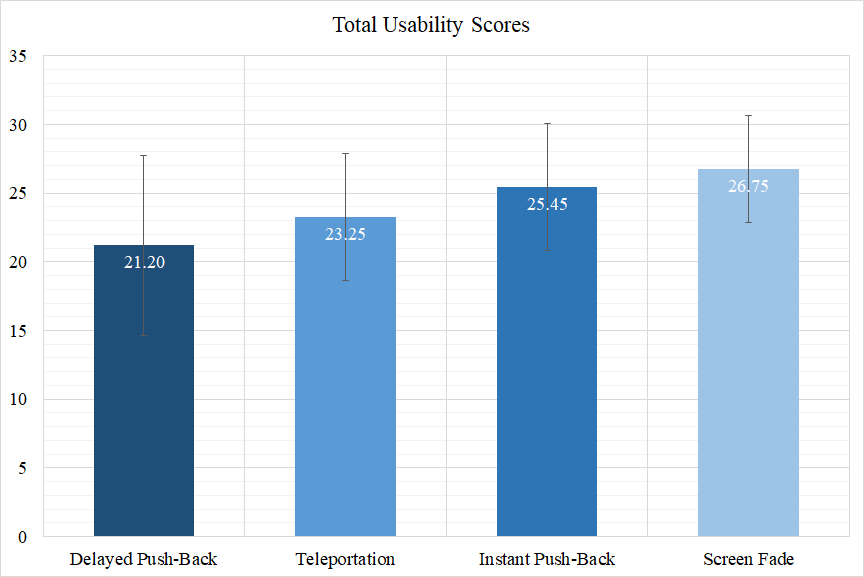
\includegraphics[width=1\textwidth]{img/total_usability_scores.png}
\caption{The total usability scores.}
\label{fig:total_usability_scores}
\end{figure}
